\newpage
\subsection{Actividad 6}
Aplicar \textsc{ltiview} al sistema servomotor de posición en
bucle cerrado discretizado con ganancia $k_a=1$ y calcular las
especificaciones de respuesta transitoria (t\_subida, t\_pico,
t\_establecimiento, sobreoscilación) ante entrada escalón unitario.
\begin{tcolorbox}[sharp corners, colframe=bluebox, title= Sistema
  servomotor de posición.,breakable=unlimited]
  $>>>$ transient\_ans = kr*feedback(Gposicionz,kr)\\
  $>>>$ ltiview(\textcolor{blue}{`step'},transient\_ans)
  \vspace*{0.35em}
  \begin{tcolorbox}[sharp corners, colback = white]
    \color{gray}
\begin{verbatim}
transient_ans =
 
  0.006147 z^2 + 0.01251 z + 0.001159
  ------------------------------------
  z^3 - 1.795 z^2 + 0.8456 z - 0.03052
 
Sample time: 0.05 seconds
Discrete-time transfer function.
\end{verbatim}
  \end{tcolorbox}%
  \vspace*{0.5em}
  \mkanscode{
\begin{figure}[H]
  \centering
  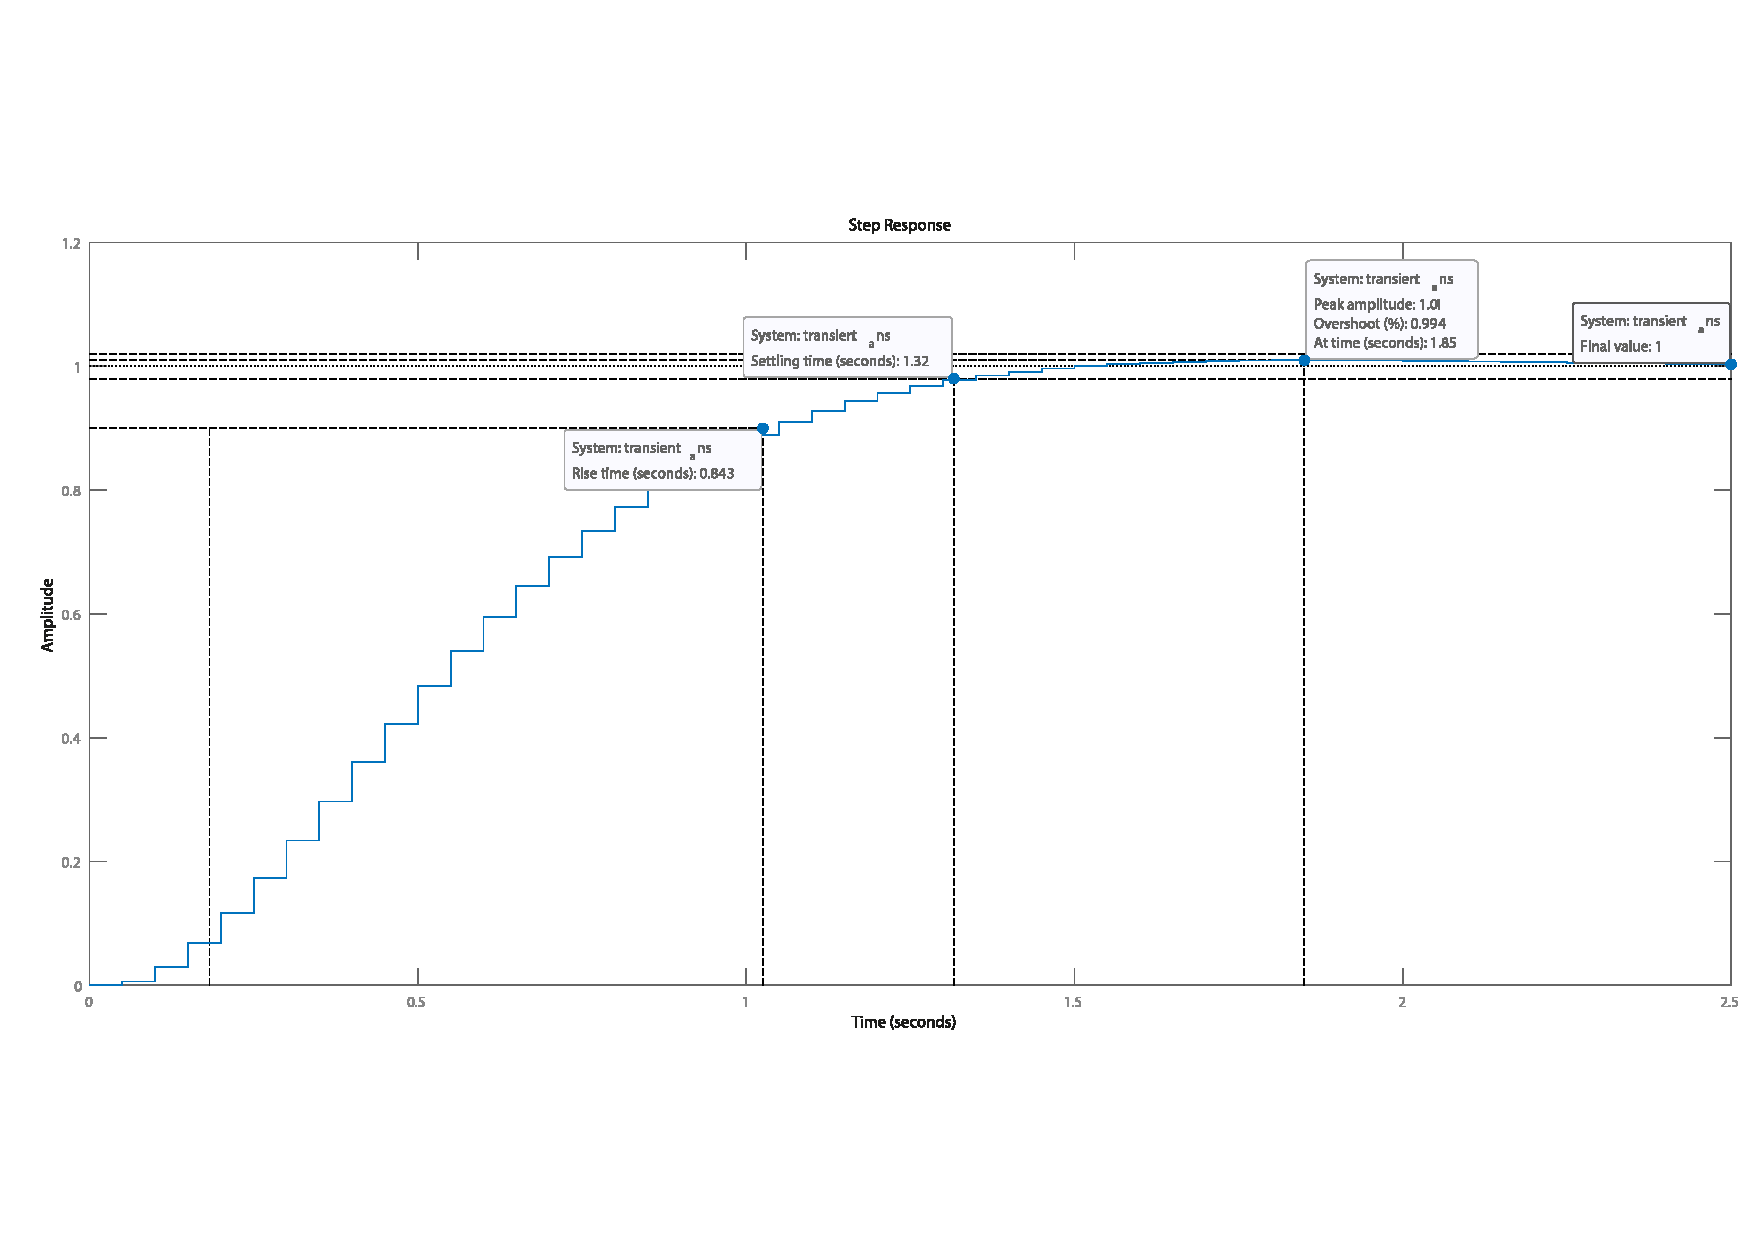
\includegraphics[clip, trim=0.5cm 3.5cm 0.35cm 3.7cm,
  scale=0.48]{images/figura 2.pdf}
  % izquierda,abajo,derecha,arriba
  \caption{Especificaciones de respuesta transitoria en bucle cerrado.}
    \label{fig:comparacion}
\end{figure}
}
\end{tcolorbox}%
